\documentclass{standalone}[]

\usepackage{tikz}
\usepackage{pgfplots}
\usepgfplotslibrary{statistics}
\usetikzlibrary{pgfplots.statistics}
\usepackage{etoolbox}

\newtoggle{label}
\togglefalse{label}
\pgfplotsset{compat=1.12}

\begin{document}

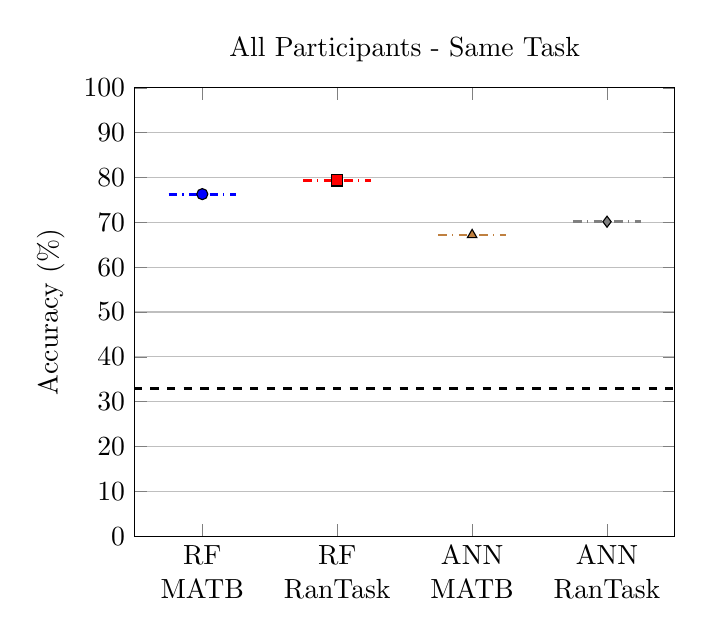
\begin{tikzpicture}
\begin{axis}[
	ymajorgrids,
	ytick={0,10,...,100},
	scatter/classes= {
		a={mark=*, black, fill=blue},
		b={mark=square*, black, fill=red},
		c={mark=triangle*, black, fill=brown},
		d={mark=diamond*, black, fill=gray}
	},
	xtick={1,2,3,4},
	xticklabel style={align=center},
	xticklabels={RF\\MATB, RF\\RanTask, ANN\\MATB, ANN\\RanTask},
	title=All Participants - Same Task, 
	ylabel=Accuracy (\%),
	ymin=0,
	ymax=100,
	xmin = .5, 
	xmax=4.5,]

		\addplot+[ mark=None, dashed, black, line width = 1pt ]
	coordinates {
	(0, 33)
	(5, 33)	
};

	\addplot+[ scatter,
			only marks,
			scatter src=explicit symbolic]
	 coordinates { 
		(1,76.30) [a]
		(2,79.35) [b]
		(3,67.20) [c]
		(4,70.15) [d]
	};
	
\addplot+[ mark=None, dashdotted, blue, line width = 1pt ] 
	coordinates {
		(0.75, 76.30)
		(1.25, 76.30)
};

\addplot+[ mark=None, dashdotted, red, line width = 1pt ] 
	coordinates {
		(1.75, 79.35)
		(2.25, 79.35)
};

\addplot+[ mark=None, dashdotted, brown, line width = 1pt ] 
	coordinates {
		(2.75, 67.20)
		(3.25, 67.20)
};

\addplot+[ mark=None, dashdotted, gray, line width = 1pt ] 
	coordinates {
		(3.75, 70.15)
		(4.25, 70.15)
};
	
\end{axis}
\end{tikzpicture}

\end{document}
















